\documentclass[a4paper]{article}

\usepackage[portuguese]{babel}
\usepackage[utf8]{inputenc}
\usepackage{amsmath}
\usepackage{graphicx}
\usepackage[colorinlistoftodos]{todonotes}
\usepackage{amssymb}
\usepackage{relsize}
\usepackage{MnSymbol}
\newcommand{\diff}{\mathrm{d}}
\newcommand{\bd}{\mathrm{bd}\,}
\newcommand{\cl}{\mathrm{cl}\,}
\newcommand{\ext}{\mathrm{ext}\,}
\newcommand{\intr}{\mathrm{int}\,}



\title{Segundo e terceiro trabalhos pr\'aticos }

\author{Herberth Amaral}


\begin{document}
\maketitle
\section*{Trabalho 2 - Quest\~ao 2}

Registro dos treinamentos:

\begin{center}
\begin{tabular}{|c|c|c|c|c|c|c|c|}
\hline
Treinamento & Erro quadr\'atico m\'edio & N\'umero total de \'epocas  \\ \hline
$\texttt{T1}$ & 0.0023 & 181  \\ \hline
$\texttt{T2}$ & 0.0016 & 166  \\ \hline
$\texttt{T3}$ & 0.0020 & 168  \\ \hline
$\texttt{T4}$ & 0.0022 & 179  \\ \hline
$\texttt{T5}$ & 0.0017 & 187  \\ \hline
\end{tabular}
\end{center}

\section*{Trabalho 2 - Quest\~ao 3}

\texttt{T1 - 181 \'epocas:}

\includegraphics[width=\textwidth]{T1.png}

\paragraph{}
\texttt{T5 - 187 \'epocas:}

\includegraphics[width=\textwidth]{T5.png}

\section*{Trabalho 2 - Quest\~ao 4}

Toda varia\c{c}\~ao de \textit{performance} nas redes neurais implementadas neste trabalho d\'a-se ao fato da escolha aleat\'oria dos pesos inciais dos neur\^onios. Pode-se comprovar esta afirma\c{c}ao setando os pesos iniciais da rede com valores fixos e executando treinamentos. Todos os treinamentos utilizar\~ao o mesmo número de \'epocas e dar\~ao o mesmo resultado todas as vezes que for executado.

Isso acontece porque o treinamento em si das redes n\~ao envolve aleatoriedade, portanto s\~ao determin\'isticos. A \'unica aleatoridade presente no processo \'e na escolha dos pesos iniciais.


\section*{Trabalho 2 - Quest\~ao 5}

\begin{tabular}{|c|c|c|c|c|c|c|c|c|c|}
\hline
$Amostra$ & $x_1$ & $x_2$ & $x_3$ & $d$ & $T1$ & $T2$ & $T3$ & $T4$ & $T5$ \\ \hline
$1$  & 0,0611 & 0,2860 & 0,7464 & 0,4831 & 0.5294 & 0.4665 & 0.5683 & 0.4450 & 0.5285 \\ \hline
$2$  & 0,5102 & 0,7464 & 0,0860 & 0,5965 & 0.5360 & 0.6754 & 0.5299 & 0.5905 & 0.6547 \\ \hline
$3$  & 0,0004 & 0,6916 & 0,5006 & 0,5318 & 0.6313 & 0.5464 & 0.5164 & 0.5689 & 0.4923 \\ \hline
$4$  & 0,9430 & 0,4476 & 0,2648 & 0,6843 & 0.6734 & 0.6345 & 0.7079 & 0.6816 & 0.7329 \\ \hline
$5$  & 0,1399 & 0,1610 & 0,2477 & 0,2872 & 0.2682 & 0.3591 & 0.2369 & 0.3187 & 0.3006 \\ \hline
$6$  & 0,6423 & 0,3229 & 0,8567 & 0,7663 & 0.7228 & 0.7951 & 0.7024 & 0.7997 & 0.8260 \\ \hline
$7$  & 0,6492 & 0,0007 & 0,6422 & 0,5666 & 0.5171 & 0.5448 & 0.5708 & 0.5597 & 0.4831 \\ \hline
$8$  & 0,1818 & 0,5078 & 0,9046 & 0,6601 & 0.6985 & 0.6759 & 0.6567 & 0.6265 & 0.7243 \\ \hline
$9$  & 0,7382 & 0,2647 & 0,1916 & 0,5427 & 0.5544 & 0.5293 & 0.5397 & 0.4646 & 0.5203 \\ \hline
$10$ & 0,3879 & 0,1307 & 0,8656 & 0,5836 & 0.5648 & 0.5747 & 0.6308 & 0.5369 & 0.6129 \\ \hline
$11$ & 0,1903 & 0,6523 & 0,7820 & 0,6950 & 0.6559 & 0.7098 & 0.6684 & 0.6572 & 0.7292 \\ \hline
$12$ & 0,8401 & 0,4490 & 0,2719 & 0,6790 & 0.6535 & 0.6762 & 0.6661 & 0.6367 & 0.7125 \\ \hline
$13$ & 0,0029 & 0,3264 & 0,2476 & 0,2956 & 0.3025 & 0.3749 & 0.2153 & 0.3441 & 0.3274 \\ \hline
$14$ & 0,7088 & 0,9342 & 0,2763 & 0,7742 & 0.7579 & 0.8647 & 0.8696 & 0.8012 & 0.8694 \\ \hline
$15$ & 0,1283 & 0,1882 & 0,7253 & 0,4662 & 0.5297 & 0.4357 & 0.5632 & 0.4281 & 0.4988 \\ \hline
$16$ & 0,8882 & 0,3077 & 0,8931 & 0,8093 & 0.7836 & 0.8593 & 0.8460 & 0.8527 & 0.8469 \\ \hline
$17$ & 0,2225 & 0,9182 & 0,7820 & 0,7581 & 0.6910 & 0.7038 & 0.7847 & 0.7867 & 0.7719 \\ \hline
$18$ & 0,1957 & 0,8423 & 0,3085 & 0,5826 & 0.6256 & 0.5794 & 0.5960 & 0.5941 & 0.5269 \\ \hline
$19$ & 0,9991 & 0,5914 & 0,3933 & 0,7938 & 0.8511 & 0.6883 & 0.8028 & 0.8478 & 0.8121 \\ \hline
$20$ & 0,2299 & 0,1524 & 0,7353 & 0,5012 & 0.5546 & 0.4717 & 0.5844 & 0.4600 & 0.5178 \\ \hline
\multicolumn{5}{|c|}{Erro relativo m\'edio \%}& 6.3116 & 6.1923 & 6.2223 & 5.3116 & 6.7596 \\ \hline
\multicolumn{5}{|c|}{Vari\^ancia \%}& 0.2214 & 0.2562 & 0.2868 & 0.1551 & 0.1843 \\ \hline
\end{tabular}

\section*{Trabalho 2 - Quest\~ao 6}

Baseado nos dados da quest\~ao 5, \'e poss\'ivel concluir que o T4 possui melhor generaliza\c{c}ao por possuir menor erro nos dados de valida\c{c}\~ao.


\section*{Trabalho 3 - Quest\~ao 3}

Segue abaixo as figuras de todos os treinamentos. Por motivos alheios à minha compreensão, o MATLAB não mantém os valores que configurei para setar o erro esperado e o número de épocas, portanto o padrão de épocas ficou com o valor 1000, em que o tempo de execução entre um tipo de algoritmo e outro é desprezível (\textless 1s).
\subsection*{Treinamentos com gradiente descendente sem momentum}
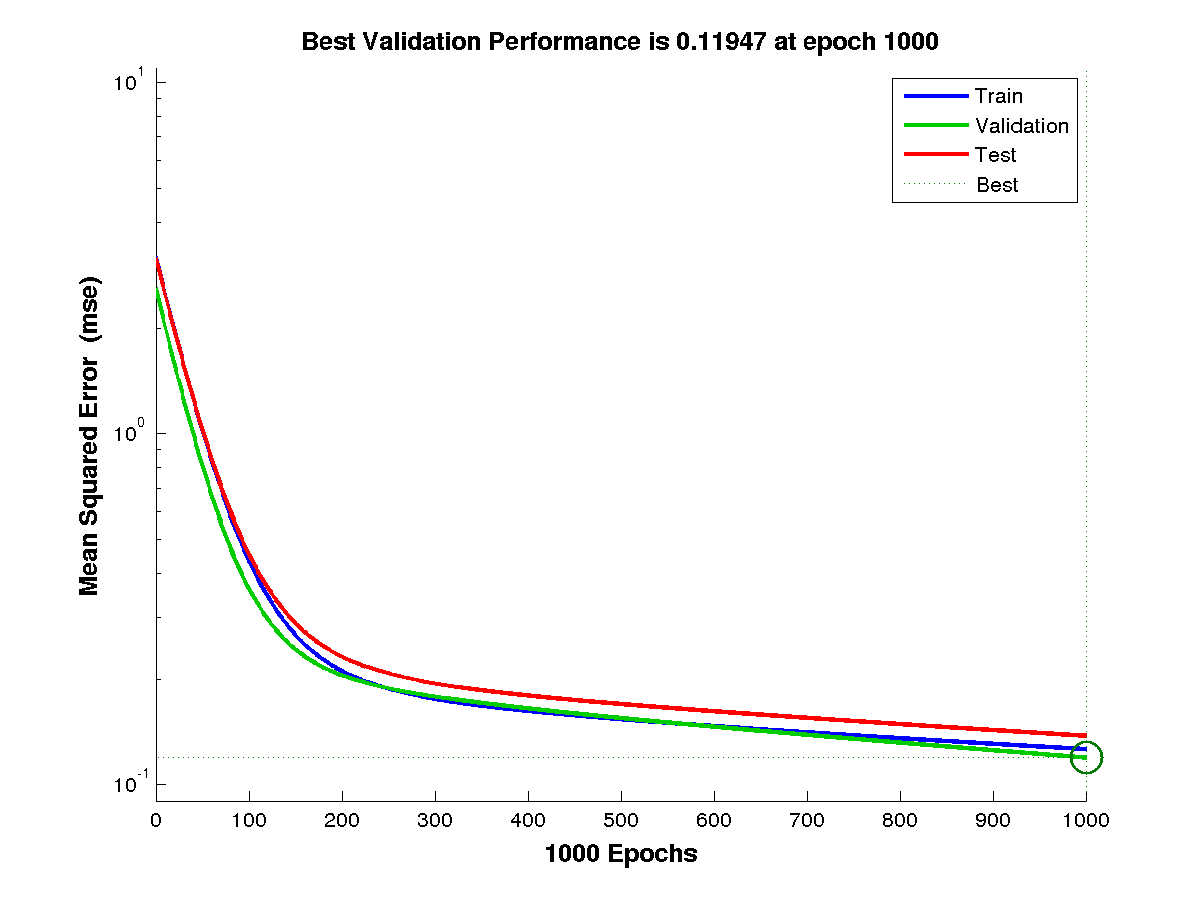
\includegraphics[width=\textwidth]{tr1.png}
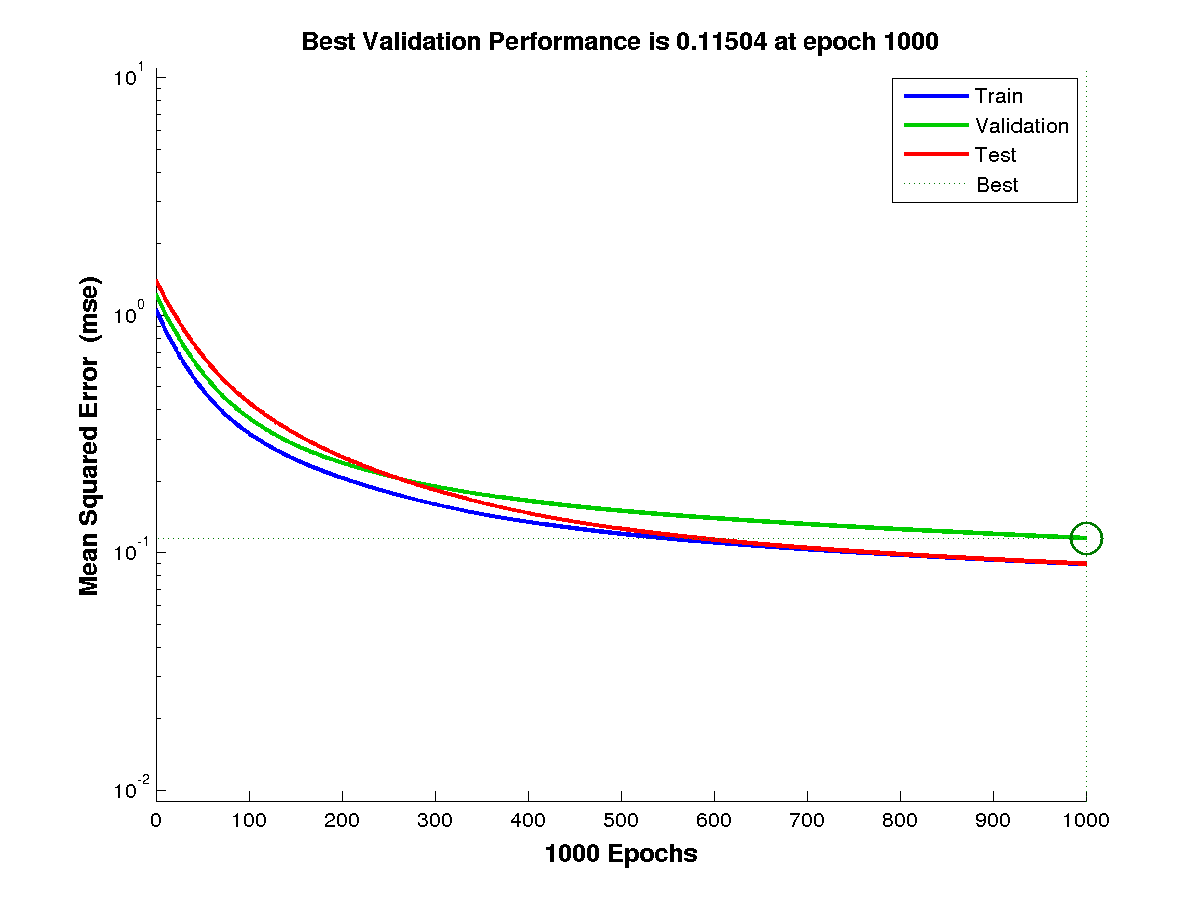
\includegraphics[width=\textwidth]{tr2.png}
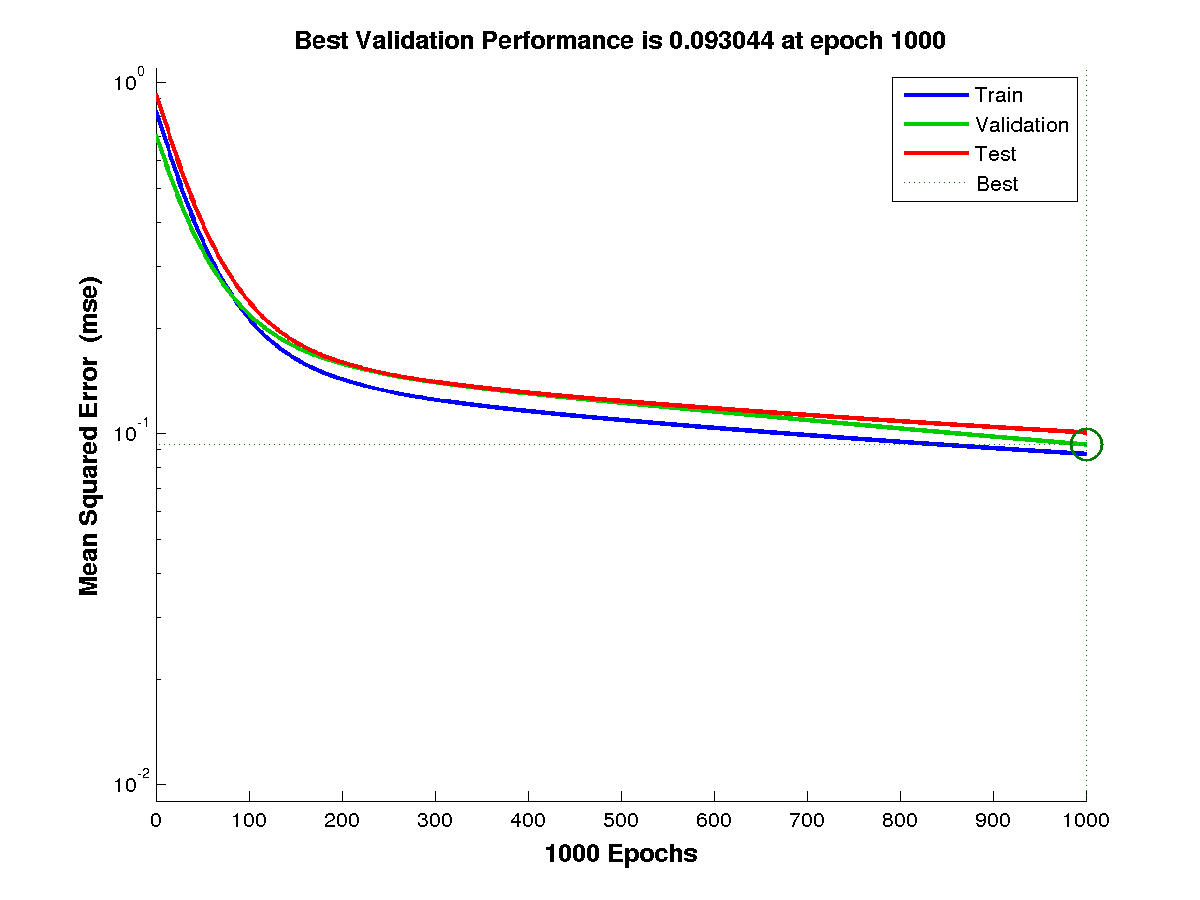
\includegraphics[width=\textwidth]{tr3.png}
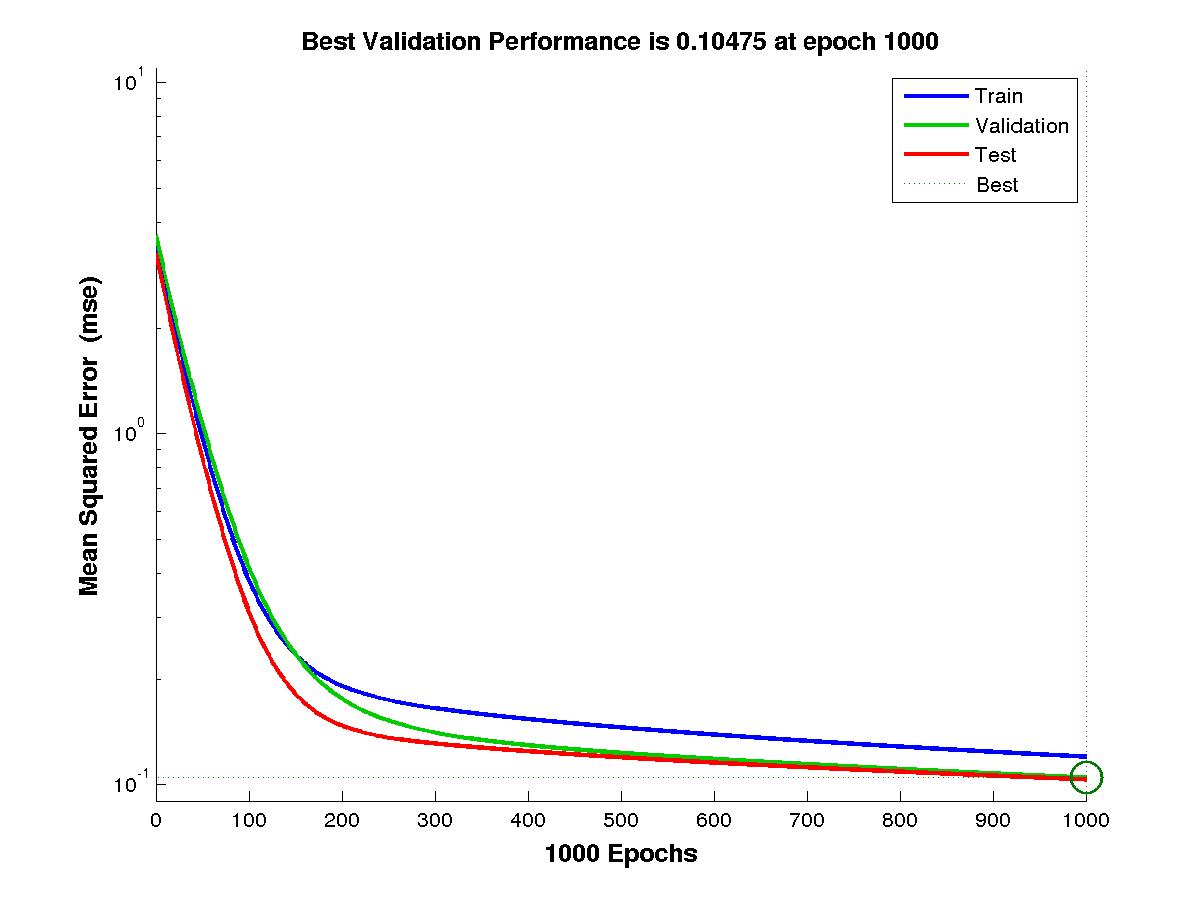
\includegraphics[width=\textwidth]{tr4.png}
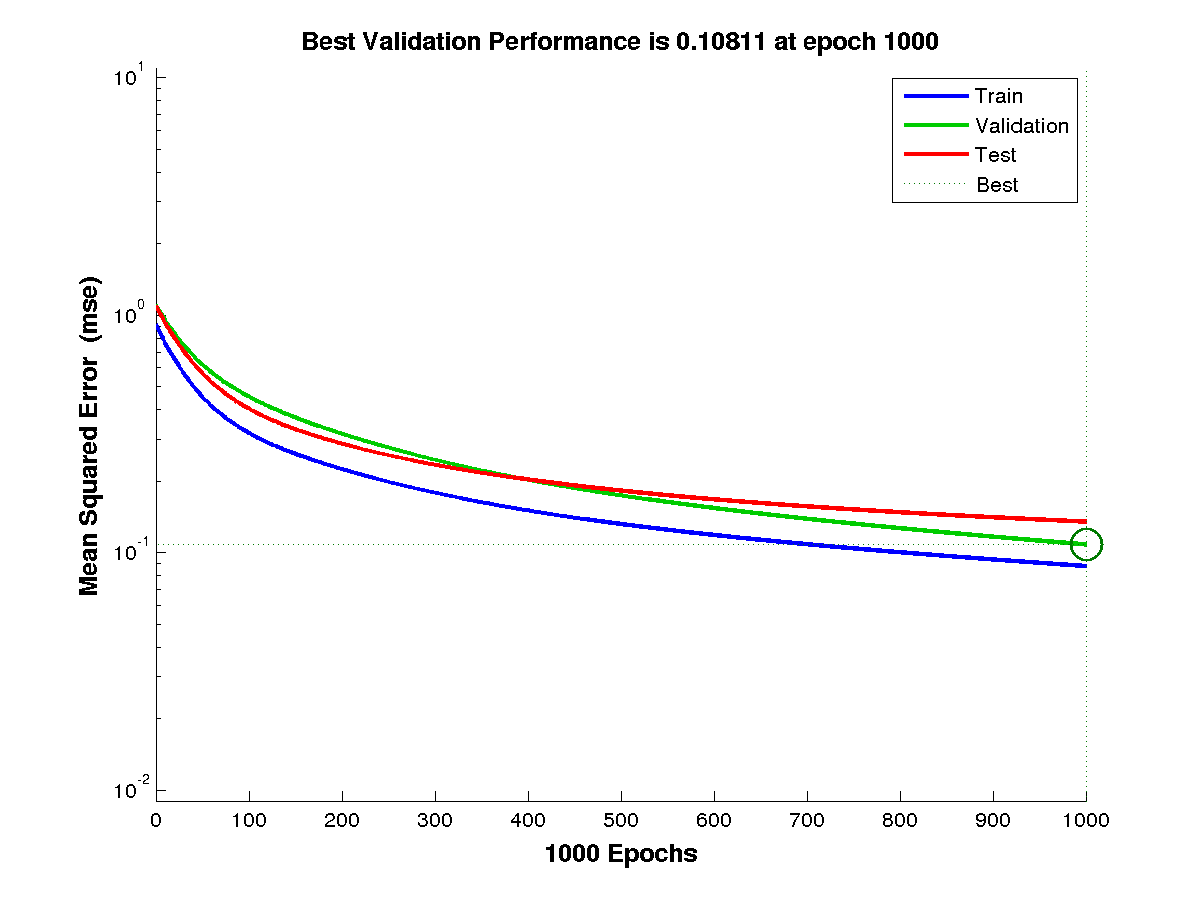
\includegraphics[width=\textwidth]{tr5.png}
\subsection*{Treinamentos com gradiente descendente com momentum}
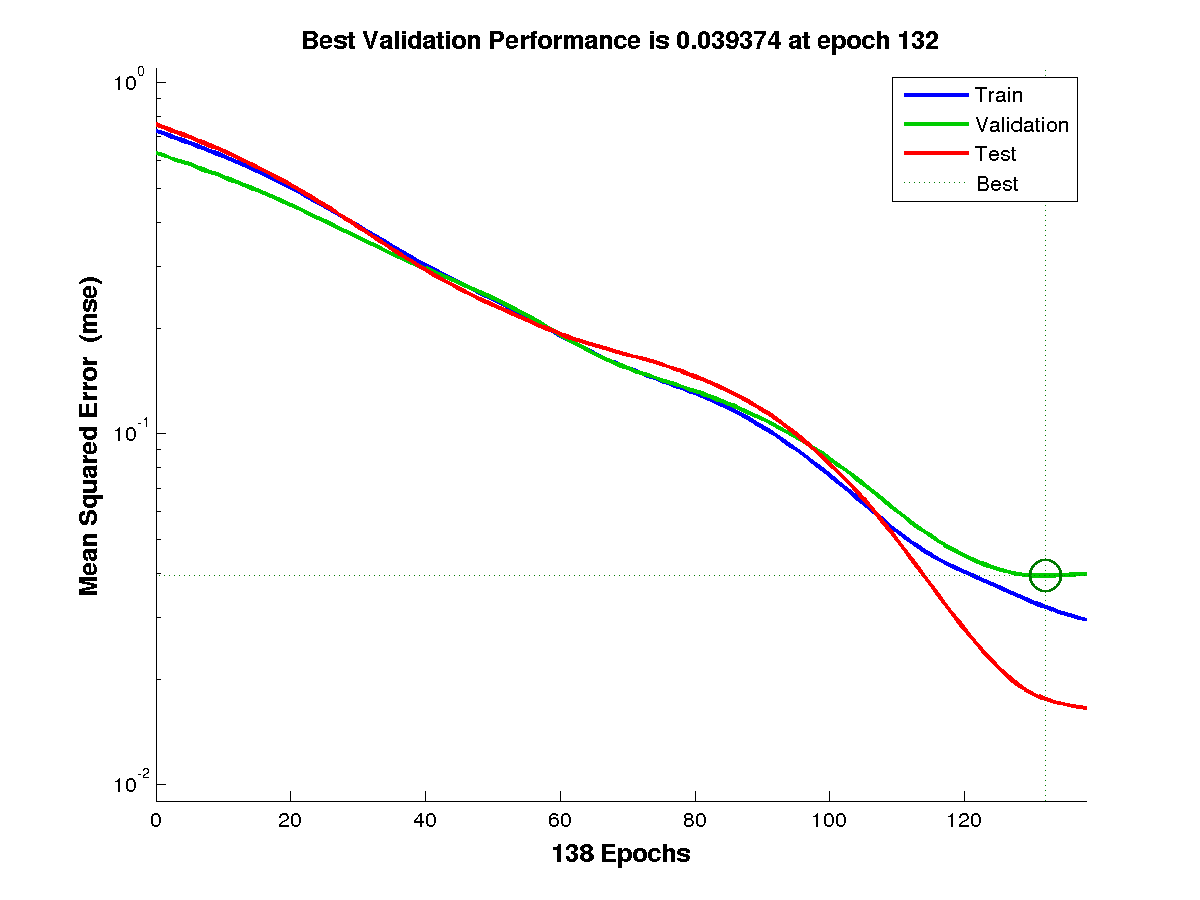
\includegraphics[width=\textwidth]{tr1m.png}
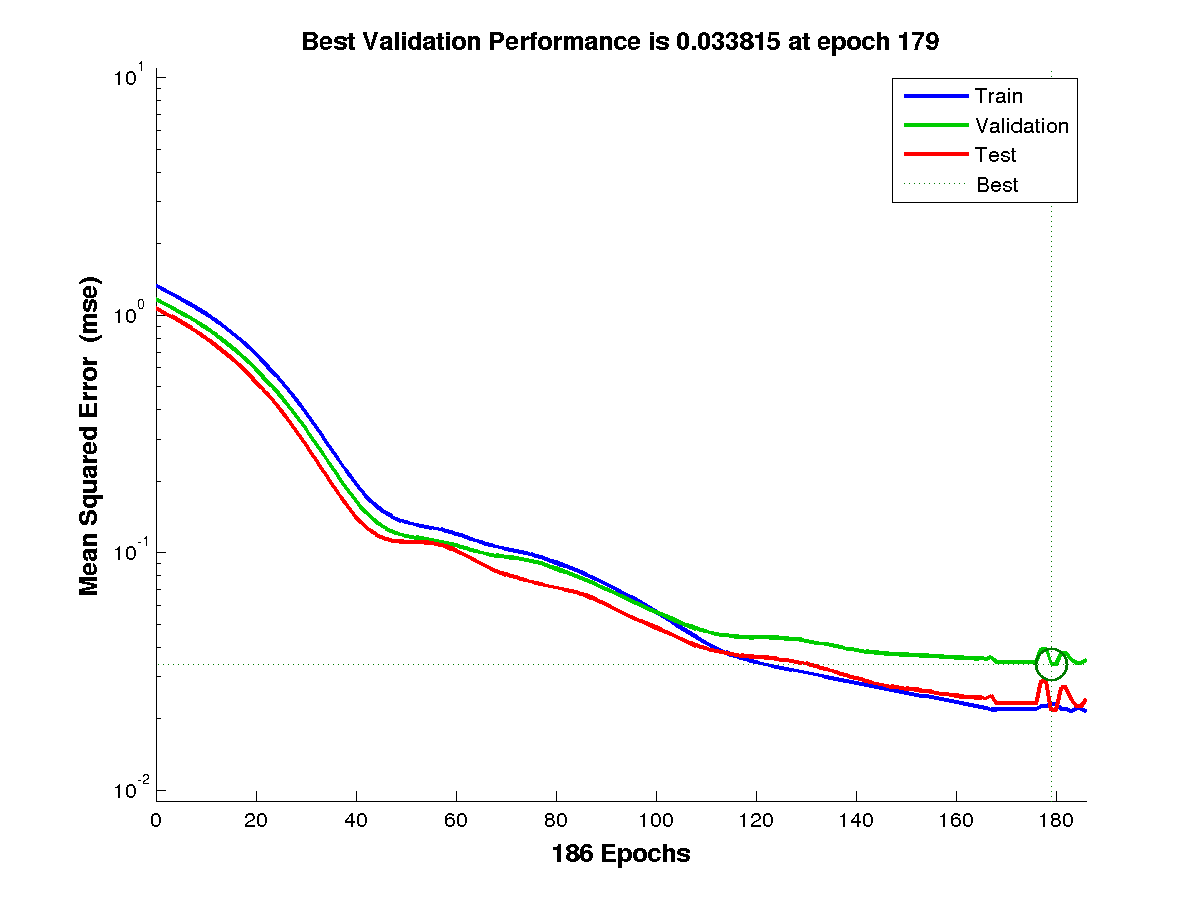
\includegraphics[width=\textwidth]{tr2m.png}
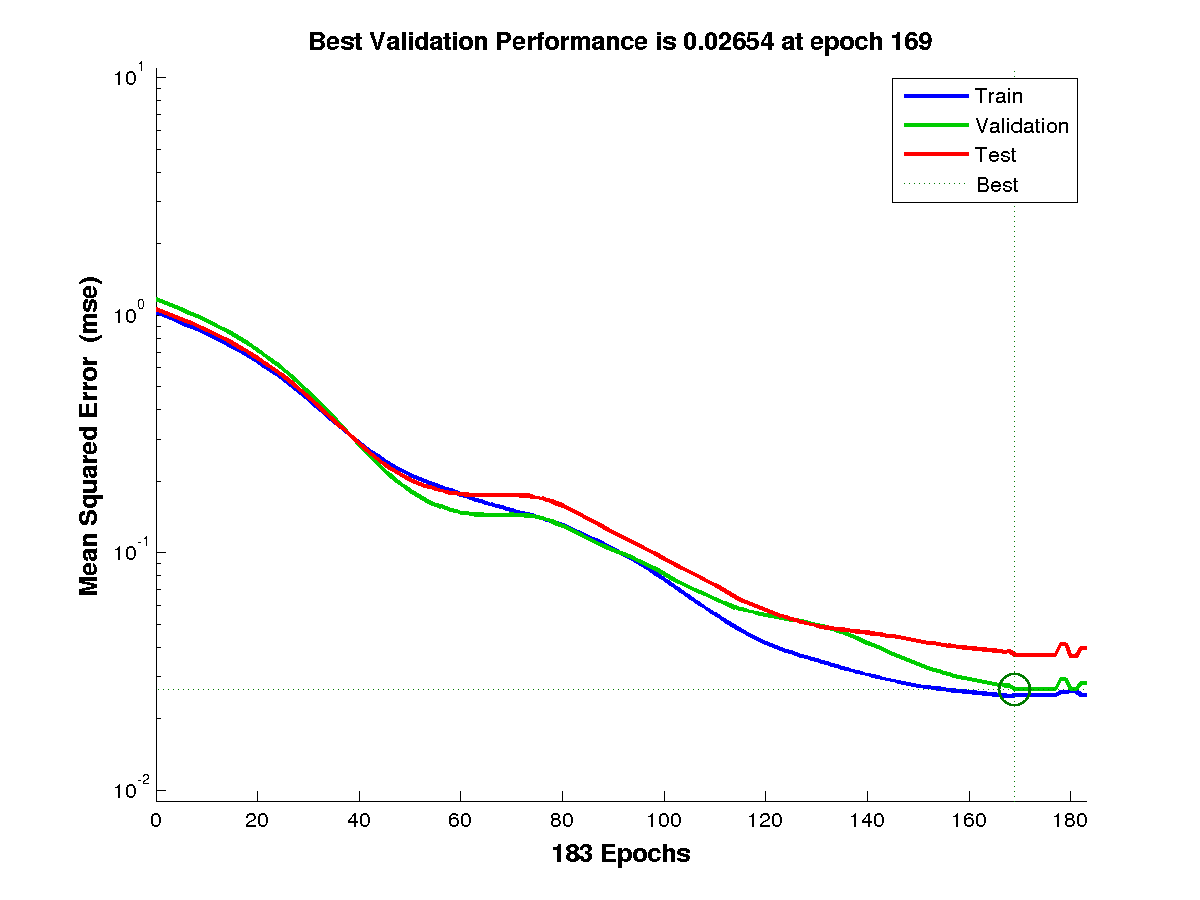
\includegraphics[width=\textwidth]{tr3m.png}
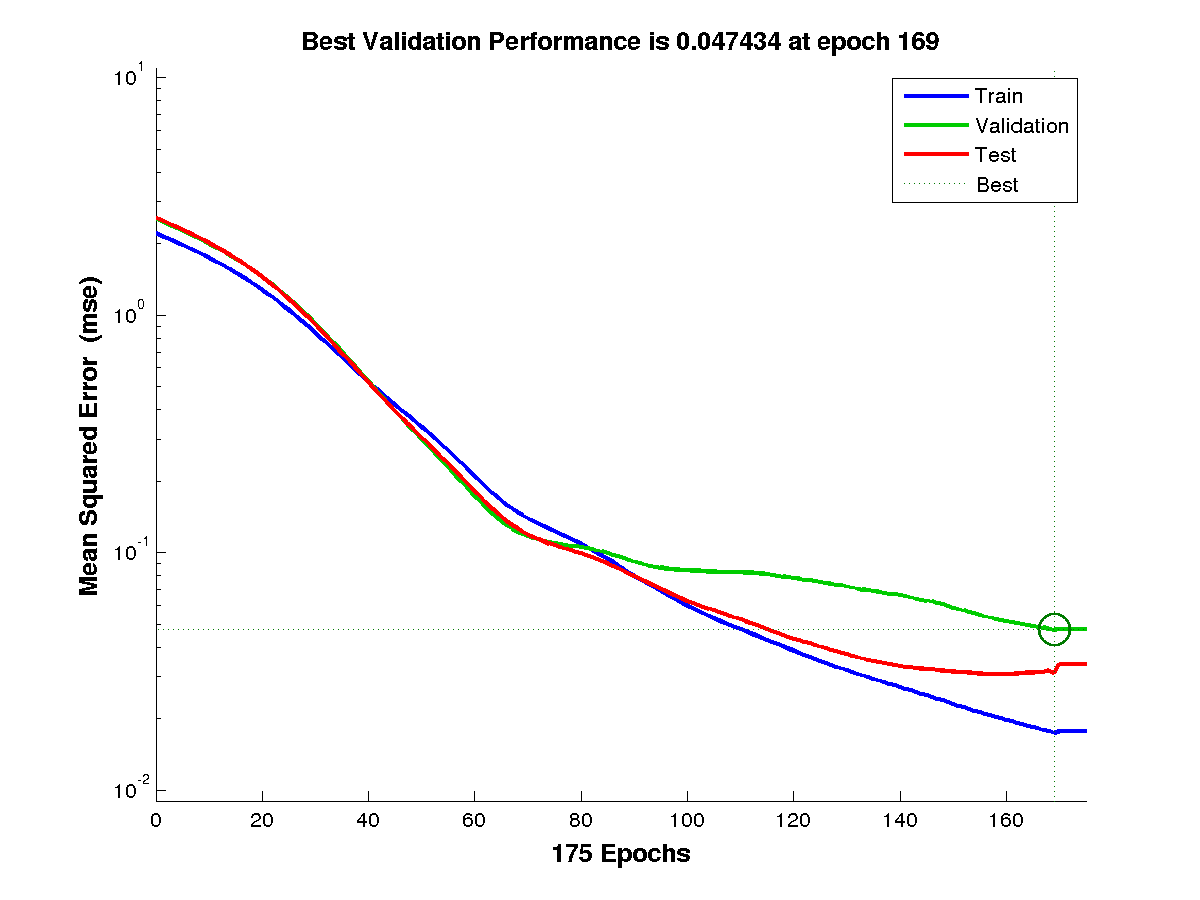
\includegraphics[width=\textwidth]{tr4m.png}
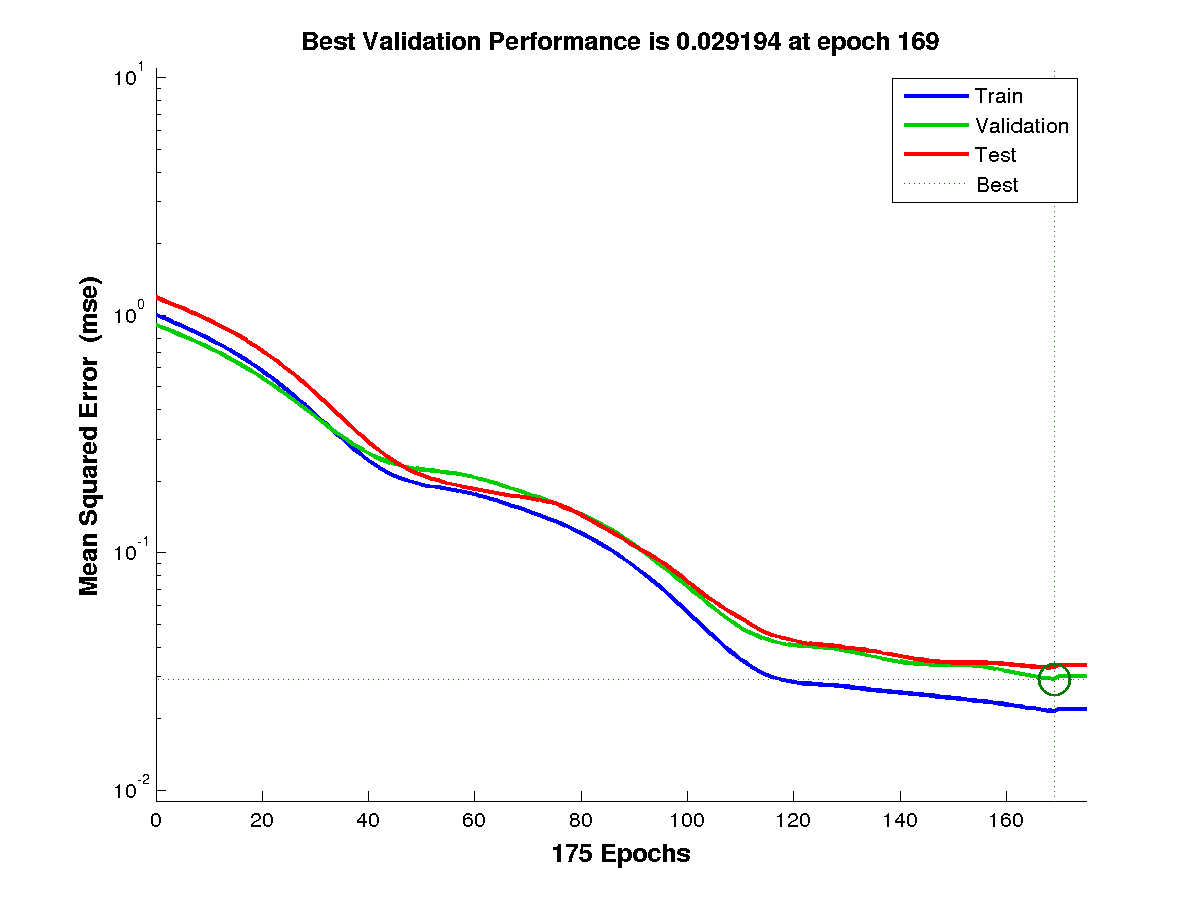
\includegraphics[width=\textwidth]{tr5m.png}

\section*{Trabalho 3 - Quest\~ao 5}

\begin{center}
\begin{tabular}{|c|c|c|c|c|c|c|c|c|c|}
\hline
$Amostra$ & $x_1$ & $x_2$ & $x_3$ & $d_1$ & $d_2$ & $d_3$ & $y_1$ & $y_2$ & $y_3$ \\ \hline
$0.8622$ & 0.7101 & 0.6236 & 0.7894 & 0 & 0 & 1 & 0 & 0 & 1 \\ \hline
$0.2741$ & 0.1552 & 0.1333 & 0.1516 & 1 & 0 & 0 & 1 & 0 & 0 \\ \hline
$0.6772$ & 0.8516 & 0.6543 & 0.7573 & 0 & 0 & 1 & 0 & 0 & 1 \\ \hline
$0.2178$ & 0.5039 & 0.6415 & 0.5039 & 0 & 1 & 0 & 0 & 1 & 0 \\ \hline
$0.7260$ & 0.7500 & 0.7007 & 0.4953 & 0 & 0 & 1 & 0 & 0 & 1 \\ \hline
$0.2473$ & 0.2941 & 0.4248 & 0.3087 & 1 & 0 & 0 & 0 & 0 & 0 \\ \hline
$0.5682$ & 0.5683 & 0.5054 & 0.4426 & 0 & 1 & 0 & 0 & 1 & 0 \\ \hline
$0.6566$ & 0.6715 & 0.4952 & 0.3951 & 0 & 1 & 0 & 0 & 1 & 0 \\ \hline
$0.0705$ & 0.4717 & 0.2921 & 0.2954 & 1 & 0 & 0 & 1 & 0 & 0 \\ \hline
$0.1187$ & 0.2568 & 0.3140 & 0.3037 & 1 & 0 & 0 & 0 & 0 & 0 \\ \hline
$0.5673$ & 0.7011 & 0.4083 & 0.5552 & 0 & 1 & 0 & 0 & 1 & 0 \\ \hline
$0.3164$ & 0.2251 & 0.3526 & 0.2560 & 1 & 0 & 0 & 1 & 0 & 0 \\ \hline
$0.7884$ & 0.9568 & 0.6825 & 0.6398 & 0 & 0 & 1 & 0 & 0 & 1 \\ \hline
$0.9633$ & 0.7850 & 0.6777 & 0.6059 & 0 & 0 & 1 & 0 & 0 & 1 \\ \hline
$0.7739$ & 0.8505 & 0.7934 & 0.6626 & 0 & 0 & 1 & 0 & 0 & 1 \\ \hline
$0.4219$ & 0.4136 & 0.1408 & 0.0940 & 1 & 0 & 0 & 1 & 0 & 0 \\ \hline
$0.6616$ & 0.4365 & 0.6597 & 0.8129 & 0 & 0 & 1 & 0 & 1 & 0 \\ \hline
$0.7325$ & 0.4761 & 0.3888 & 0.5683 & 0 & 1 & 0 & 0 & 1 & 0 \\ \hline
\multicolumn{7}{|c|}{Total de acertos (\%)} & \multicolumn{3}{|c|}{83.3\%} \\ \hline
\end{tabular}
\end{center}


\end{document}
